  \solution{
Implication graph:\medskip

%TCIMACRO{%
%\TeXButton{Decision tree}{\begin{tikzpicture}[node distance=2.5cm,auto]
%\node (A) {A=0@1};
%\node (B) [right of=A] {B=1@1};
%\node (D) [right of=B] {D=0@3};
%\node (G) [right of=D] {G=0@3};
%\node (H) [below of=G] {H=1@3};
%\node (K) [right of=H] {$\mathcal K$};
%\node (E) [above of=D] {E=0@3};
%\node (F) [right of=E] {F=1@3};
%\node (J) [right of=G] {J=1@3};
%\node (C) [above of=J] {C=1@2};
%\path[->] (A) edge node {$C_1$} (B);
%\path[->] (B) edge node {$C_3$} (D);
%\path[->] (D) edge node {$C_5$} (G);
%\path[->] (G) edge node {$C_2$} (H);
%\path[->] (H) edge node {$C_7$} (K);
%\path[->] (A) edge node {$C_2$} (H);
%\path[->] (C) edge node {$C_6$} (J);
%\path[->] (J) edge node {$C_7$} (K);
%\path[->] (E) edge node {$C_3$} (D);
%\path[->] (E) edge node {$C_4$} (F);
%\path[->] (F) edge node {$C_5$} (G);
%\path[->] (G) edge node {$C_6$} (J);
%\end{tikzpicture}}}%
%BeginExpansion
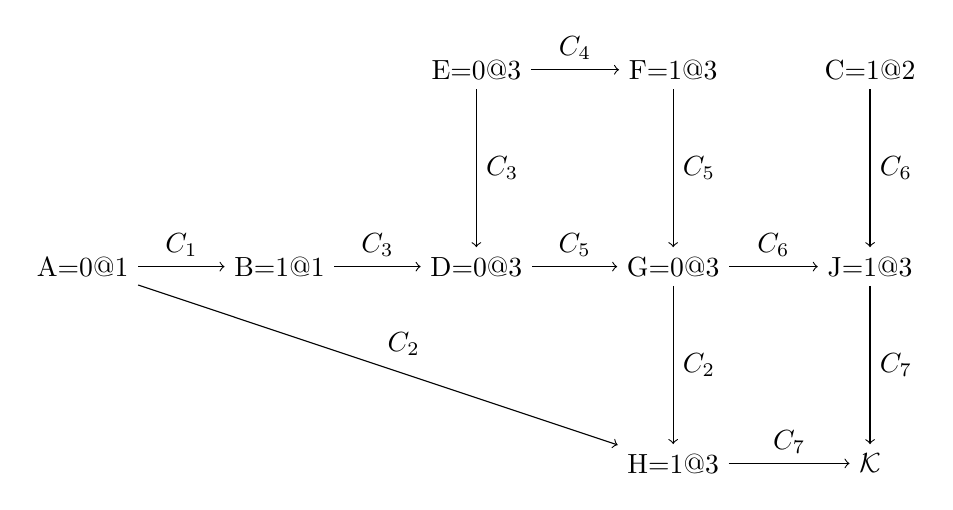
\begin{tikzpicture}[node distance=2.5cm,auto]
\node (A) {A=0@1};
\node (B) [right of=A] {B=1@1};
\node (D) [right of=B] {D=0@3};
\node (G) [right of=D] {G=0@3};
\node (H) [below of=G] {H=1@3};
\node (K) [right of=H] {$\mathcal K$};
\node (E) [above of=D] {E=0@3};
\node (F) [right of=E] {F=1@3};
\node (J) [right of=G] {J=1@3};
\node (C) [above of=J] {C=1@2};
\path[->] (G) edge node {$C_6$} (J);
\path[->] (F) edge node {$C_5$} (G);
\path[->] (C) edge node {$C_6$} (J);
\path[->] (J) edge node {$C_7$} (K);
\path[->] (E) edge node {$C_3$} (D);
\path[->] (E) edge node {$C_4$} (F);

\path[->] (A) edge node {$C_1$} (B);
\path[->] (B) edge node {$C_3$} (D);
\path[->] (D) edge node {$C_5$} (G);
\path[->] (G) edge node {$C_2$} (H);
\path[->] (H) edge node {$C_7$} (K);
\path[->] (A) edge node {$C_2$} (H);
\end{tikzpicture}%
%EndExpansion
\newline
\bigskip

  }